% This file was created by matplotlib2tikz v0.7.4.
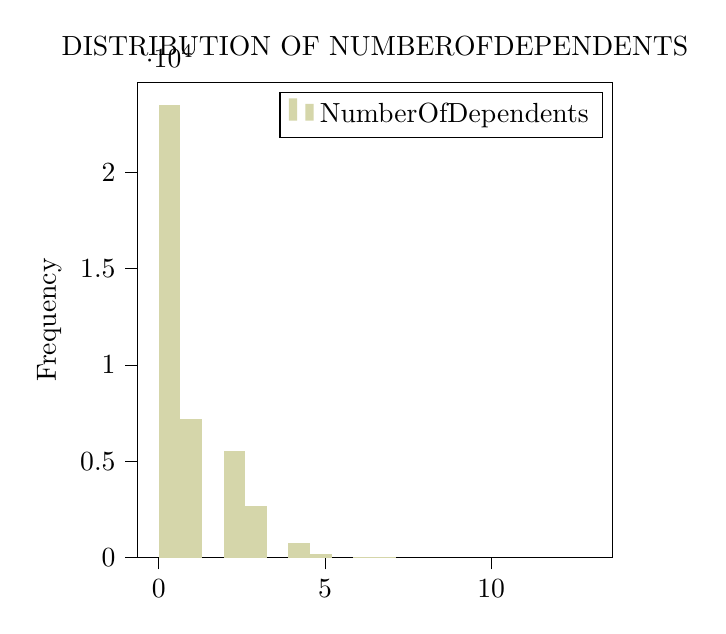
\begin{tikzpicture}

\definecolor{color0}{rgb}{0.835294117647059,0.83921568627451,0.666666666666667}

\begin{axis}[
height=3in,
tick align=outside,
tick pos=left,
title={\printsubsection{\MakeUppercase{Distribution of NumberOfDependents}}\\},
width=3in,
x grid style={white!69.01960784313725!black},
xmin=-0.65, xmax=13.65,
xtick style={color=black},
y grid style={white!69.01960784313725!black},
ylabel={Frequency},
ymin=0, ymax=24678.15,
ytick style={color=black}
]
\draw[fill=color0,draw opacity=0] (axis cs:0,0) rectangle (axis cs:0.65,23503);
\addlegendimage{ybar,ybar legend,fill=color0,draw opacity=0};
\addlegendentry{NumberOfDependents}

\draw[fill=color0,draw opacity=0] (axis cs:0.65,0) rectangle (axis cs:1.3,7211);
\draw[fill=color0,draw opacity=0] (axis cs:1.3,0) rectangle (axis cs:1.95,0);
\draw[fill=color0,draw opacity=0] (axis cs:1.95,0) rectangle (axis cs:2.6,5539);
\draw[fill=color0,draw opacity=0] (axis cs:2.6,0) rectangle (axis cs:3.25,2666);
\draw[fill=color0,draw opacity=0] (axis cs:3.25,0) rectangle (axis cs:3.9,0);
\draw[fill=color0,draw opacity=0] (axis cs:3.9,0) rectangle (axis cs:4.55,786);
\draw[fill=color0,draw opacity=0] (axis cs:4.55,0) rectangle (axis cs:5.2,201);
\draw[fill=color0,draw opacity=0] (axis cs:5.2,0) rectangle (axis cs:5.85,0);
\draw[fill=color0,draw opacity=0] (axis cs:5.85,0) rectangle (axis cs:6.5,51);
\draw[fill=color0,draw opacity=0] (axis cs:6.5,0) rectangle (axis cs:7.15,12);
\draw[fill=color0,draw opacity=0] (axis cs:7.15,0) rectangle (axis cs:7.8,0);
\draw[fill=color0,draw opacity=0] (axis cs:7.8,0) rectangle (axis cs:8.45,7);
\draw[fill=color0,draw opacity=0] (axis cs:8.45,0) rectangle (axis cs:9.1,2);
\draw[fill=color0,draw opacity=0] (axis cs:9.1,0) rectangle (axis cs:9.75,0);
\draw[fill=color0,draw opacity=0] (axis cs:9.75,0) rectangle (axis cs:10.4,0);
\draw[fill=color0,draw opacity=0] (axis cs:10.4,0) rectangle (axis cs:11.05,0);
\draw[fill=color0,draw opacity=0] (axis cs:11.05,0) rectangle (axis cs:11.7,0);
\draw[fill=color0,draw opacity=0] (axis cs:11.7,0) rectangle (axis cs:12.35,0);
\draw[fill=color0,draw opacity=0] (axis cs:12.35,0) rectangle (axis cs:13,1);
\end{axis}

\end{tikzpicture}